\documentclass[9pt,t]{beamer}
\usetheme{Madrid}
\usepackage{amsthm, hhline}
\usepackage{stmaryrd, mathtools, stmaryrd}
\usepackage{amsmath, amssymb, graphicx,array}
\usepackage{mathtools}
\DeclareMathOperator{\lcm}{lcm}
\usepackage{booktabs,comment,bbm}
\newcommand{\Z}{\mathbb{Z}}
\newcommand{\N}{\mathbb{N}}
\usepackage[english]{babel}
\usepackage[utf8x]{inputenc}
\usepackage{color}
\usepackage[export]{adjustbox}
\setbeamerfont{title in sidebar}{size=\fontsize{2}{4}\selectfont}
\setbeamerfont{author in sidebar}{size=\fontsize{2}{4}\selectfont}
\setbeamerfont{section in sidebar}{size=\fontsize{2}{4}\selectfont}
\setbeamerfont{subsection in sidebar}{size=\fontsize{2}{4}\selectfont}
\newtheorem{proposition}[theorem]{Proposition}
\fontsize{6pt}{7.2}
\DeclareMathOperator{\ex}{\mathbb{E}}
\DeclareMathOperator{\pr}{\mathbb{P}}
\DeclareMathOperator{\indic}{\mathbbm{1}}
\DeclareMathOperator{\cov}{cov}
\DeclareMathOperator{\var}{var}
\DeclareMathOperator{\sgn}{sgn}
\DeclarePairedDelimiter\ceil{\lceil}{\rceil}
\DeclarePairedDelimiter\floor{\lfloor}{\rfloor}
\DeclarePairedDelimiter\abs{\lvert}{\rvert}


\title{Asymptotics of Bernoulli Line Ensembles}

\author[Fang, Fesser, Serio, Teitler, and Wang]{Xiang Fang, Lukas Fesser, Christian Serio, Carson Teitler, and Angela Wang \\
Advisor: Evgeni Dimitrov\\
Graduate Student Assistant: Weitao Zhu}

\institute[Columbia]{Columbia University REU}

\begin{document}
	
	\begin{frame}
		\maketitle
	\end{frame}


\section{Introduction (5-6 min)}

\begin{frame}{The Gaussian universality class}
Let $\{X_i\}$ be a sequence of i.i.d. random variables, s.t. $\mathbb{E}[X_1] = \mu$, $Var(X_1^2) = \sigma^2$. Let $S_n = \sum_{i = 1}^n X_i$:

\bigskip

\begin{itemize}
\item \textbf{Law of Large Numbers:} $\frac{S_n}{n} \rightarrow \mu$ as $n \rightarrow \infty$ almost surely

\bigskip

\item \textbf{Central Limit Theorem:} $\frac{S_n - n \mu}{\sqrt{n}} \rightarrow N(0, \sigma^2)$ as $n \rightarrow \infty$

\bigskip

\item \textbf{Donsker's Theorem:} Let $S(x) = S_k$ if $x = k$ and linearly interpolate for $x \in [0, n]$ Let $\mu = 0$ and $\sigma = 1$. Then $\frac{S(n\cdot)}{\sqrt{n}} \in C([0, 1])$ and $\frac{S(n\cdot)}{\sqrt{n}} \rightarrow B(\cdot)$, where $B$ denotes a standard Brownian Motion.

\end{itemize}

\begin{figure}
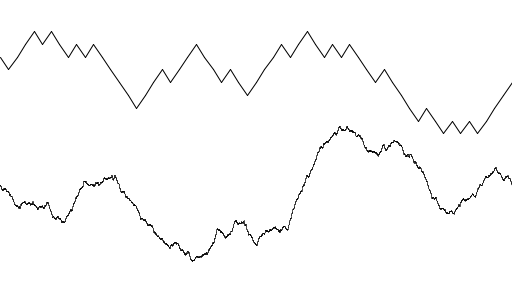
\includegraphics[height=0.5\textheight]{graphics/Gaussian.png}
\caption{An example of a Bernoulli random walk and a Brownian Motion}
\end{figure}

\end{frame}

\begin{frame}{Multiple Random Walks}
Increase the number of walkers (avoiding Bernoulli random walks and Dyson BM)
\begin{figure}
	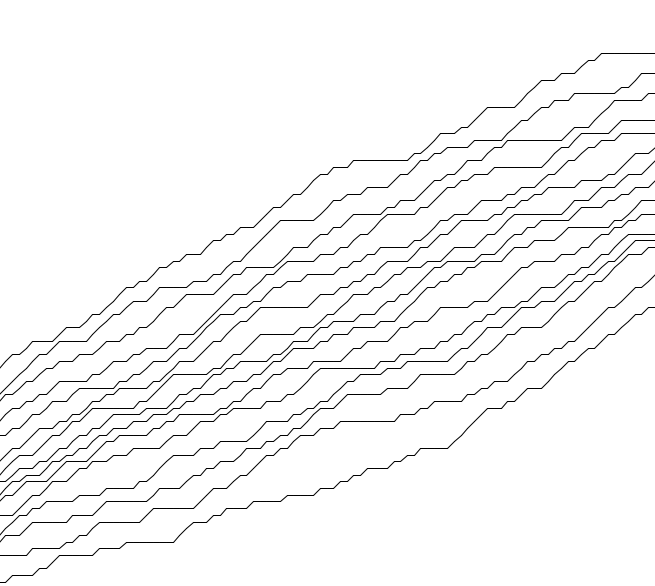
\includegraphics[height=0.25\textheight]{graphics/MultipleBernoulli.png}
	\caption{Multiple Bernoulli Random Walks}
\end{figure}
\begin{figure}
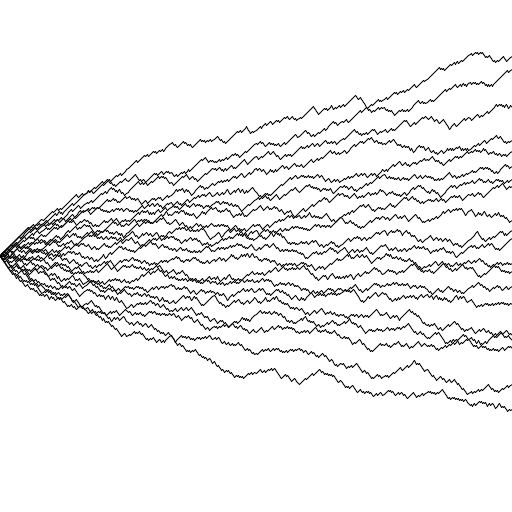
\includegraphics[height=0.25\textheight]{graphics/DysonBrownian.png}
\end{figure}
\end{frame}

\begin{frame}{Airy Line Ensemble}
What happens as N (number of walkers) goes to infinity? new type of limit occurs Airy line ensemble, top curve is the Airy process. Increasing the number of paths pushes us outside of the Gaussian universality class and into what is called the ”KPZ universality class”
\end{frame}

\begin{frame}{Open Question}
Big open problem: Show that for “generic random walks” with “generic” initial conditions we have convergence to Airy LE. This problem is open even for Bernoulli random walks (only known if all are started from 0)
\end{frame}


\section{Convergence to Airy Line Ensemble (6-7 min)}

\begin{frame}{Convergence to the Airy Line Ensemble}
	Two sufficient conditions:\begin{enumerate}
		\item Finite dimensional distribution convergence
		\item Tightness, or the existence of weak subsequential limits.
	\end{enumerate}
We focused on tightness, which requires a maximum, minimum, and conditions on the Modulus of Continuity
\begin{figure}
	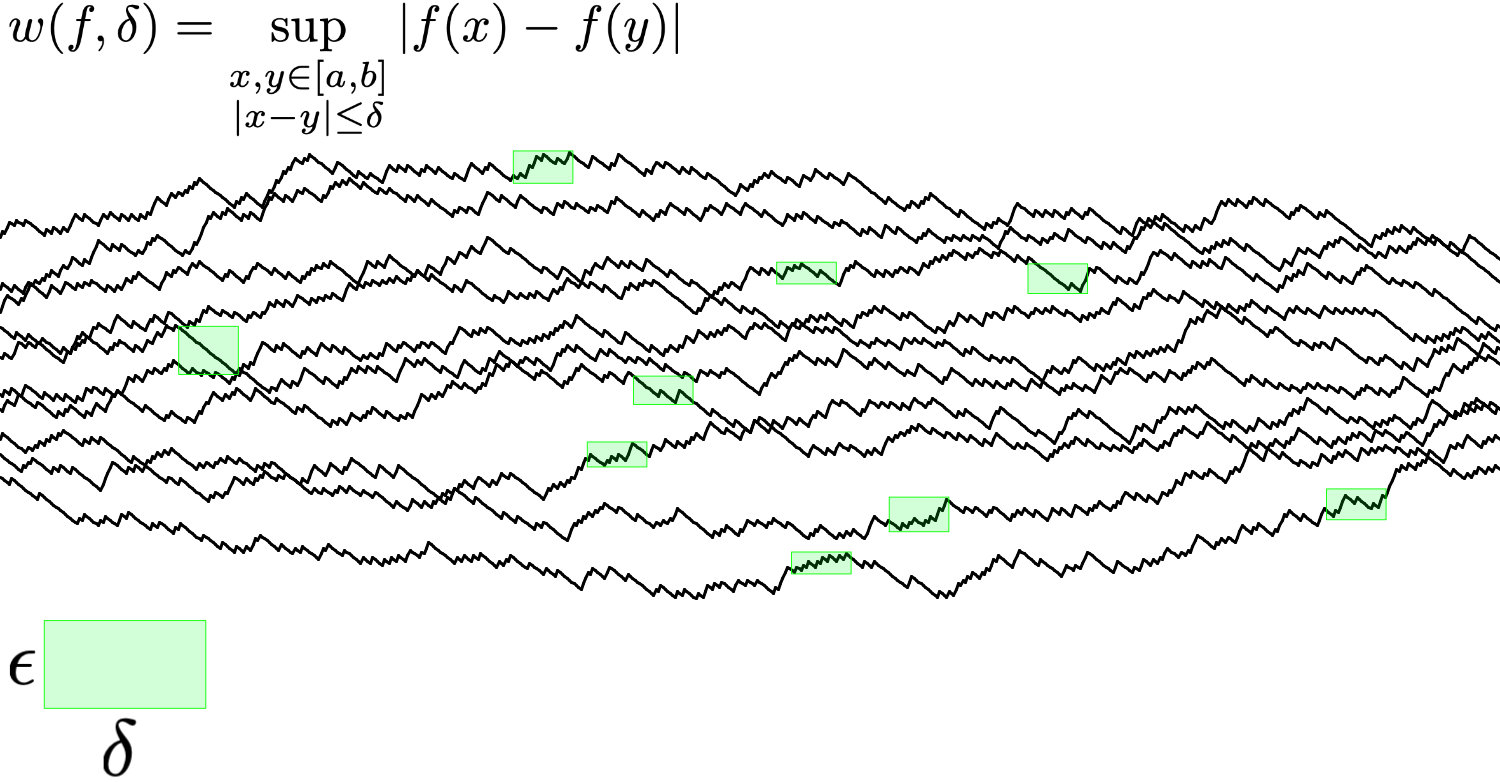
\includegraphics[height=0.55\textheight]{graphics/ModulusCont.jpg}
	\caption{The Modulus of Continuity}
\end{figure}

\end{frame}

\begin{frame}{Our Result}
\begin{theorem}With $L_1^N$ being the top curve in a Bernoulli Line Ensemble $p\in (0,1)$, and $\lambda, \alpha>0$, if for all $n\in \mathbb{Z}$,
\[\lim_{N\to\infty}P(L_1^{N}(nN^{\alpha}) - nN^{\alpha} p + \lambda n^2 N^{\alpha/2} \leq N^{\alpha/2} x) \to F_{TW}(x)\]
then the Line Ensemble is tight.
\end{theorem}
If the one-point marginal probabilities at integer times weakly converge to the Tracy Widom distribution then the Line Ensemble is tight.
\begin{figure}
	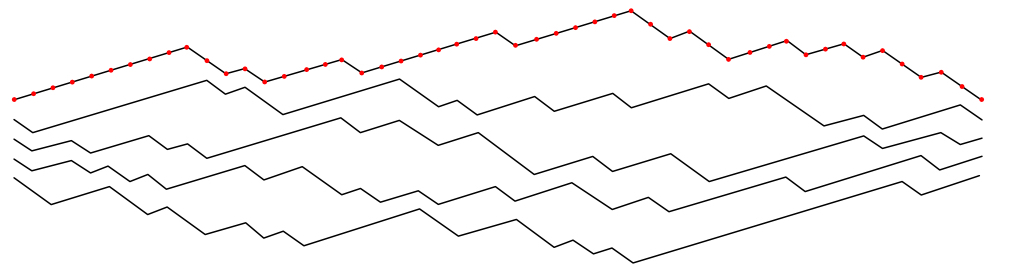
\includegraphics[width=0.75\textwidth]{graphics/ConvToTW.jpg}
	\caption{Integer time points of top line}
\end{figure}
\end{frame}

\begin{frame}{Improvements}
[Duavergne, Nica, \& Virag, 2019] - tightness assuming finite dimensional convergence to the Airy Line Ensemble. 

We achieve the same result with much less restrictive assumptions
\newline\newline\noindent
[Unsure of Image Choice]
\end{frame}


\section{Section of Paper (7-9 min)}

\begin{frame} {History of the line ensembles}
	Arguments in this paper are inspired by 
	\begin{enumerate}
		\item \textit{Brownian Gibbs property for Airy line ensembles} and \textit{KPZ line ensemble}[Corwin-Hammond ‘11, ‘13], which address the issues of {\color{red}continuous} line ensembles
		\item \textit{Transversal fluctuations of the ASEP, stochastic six vertex model, and Hall-Littlewood line ensembles} [Corwin-Dimitrov ‘17], which consider similar questions in a {\color{red}discrete} setting 
	\end{enumerate}
\end{frame}
\begin{frame}{Problem Description}
	Recall that to show tightness, we want to control \begin{enumerate}
		\item \begin{center}
			min
		\end{center}
		\item 
		\begin{center}
			max
		\end{center}
		\item 
		\begin{center}
			modulus of continuity of the line ensembles
		\end{center}
	\end{enumerate}
	We claim that for the {\color{blue}\textbf{top}} curve of our line ensemble to have a {\color{red}\textbf{parabolic shift}}, the {\color{blue}\textbf{bottom}} curve cannot dip too low, i.e. for any $r, \epsilon > 0$, there exist $R, M > 0$ such that for $N$ large enough,
	$$P( \max_{[r, R]} L_k(sN^{\alpha}) - psN^{\alpha} \leq -MN^{\alpha} ) < \epsilon$$ 
	(perhaps insert a picture)
\end{frame}
\begin{frame}
Proof  (mention monotone coupling lemmas somewhere ) - say MC with picture
2min
\end{frame}

\begin{frame}
Proof  (mention strong coupling somewhere) - say SC with picture 
L = Bernoulli bridge B is a Brownian bridge with variance. There is a probability space such that $P( sup \abs*{L - B} \geq k (\log N)^2) < \epsilon$. This is a comparison that allows for example to compare the modulus of continuity of the two. [Dimitrov-Wu ‘19]
2 min
\end{frame}

\begin{frame}{Controlling the minimum: pinning the bottom curve}
	
	\begin{lemma}[------]
		For any $r,\epsilon > 0$, there exists $R>r$ and a constant $A>0$ so that for large $N$,
		\[
		\mathbb{P}\Big(\max_{x\in[r,R]} \big(L_k^N(xN^{2/3}) - pxN^{2/3}\big) \leq -AN^{1/3}\Big) < \epsilon.
		\]
		The same is true of the maximum on $[-R,-r]$.
	\end{lemma}
	
	
	
\end{frame}

\begin{frame}{Proving the pinning lemma}
	
	\begin{itemize}
		
		\item Recall our assumption:
		\[
		\mathbb{P}\Big(\textcolor{red}{L_1^N}(nN^{2/3}) - pnN^{2/3} + \textcolor{red}{\lambda n^2} N^{1/3} \leq xN^{1/3}\Big) \underset{N\to\infty}\longrightarrow F_{TW}(x).
		\]
		
	\end{itemize}
\end{frame}


\end{document}